\section{$CO_2$ Modelling}\label{modelling}

In this section the IPCC \cite{waldron2006ipcc} methodology for calculation of emission of climate forcing gases from transportation is described. The focus of the IPCC approach is to offer methods for building national inventories for climate gas emissions. This is an attempt to summarise the key methodologies, and I will use this as a basis for developing models for single trip emissions.

\begin{table}[!ht]'
\small
  \centering
  \begin{tabular}{@{} | l|c |@{}}
    %\toprule
    %Specie & abbreviation \\ 
    %\midrule
\hline
 \multicolumn{2}{| l |}{Group 1}   \\
\hline
Carbon monoxide & CO\\ 
Nitrogen oxides & (NOx: NO and NO2)\\
Volatile organic compounds &(VOCs)\\
Methane &(CH4)\\
Non-methane VOCs &(NMVOCs)\\
Nitrous oxide &(N2O)\\
Ammonia &(NH3)\\
Particulate matter &(PM)\\
\hline
 \multicolumn{2}{| l |}{Group 2 }\\
\hline
Carbon dioxide & (CO2) \\
Sulphur dioxide & (SO2) \\
Lead & (Pb)\\
Arsenic & (As)\\ 
Cadmium & (Cd)\\ 
Chromium & (Cr) \\
Copper & (Cu)\\
Mercury & (Hg) \\
Nickel & (Ni) \\
Selenium & (Se)\\ 
Zinc & (Zn)\\
\hline
 \multicolumn{2}{| l |}{Group 3} \\
\hline
Polycyclic aromatic hydrocarbons & (PAHs) \\
Persistent organic pollutants & (POPs)\\
Polychlorinated dibenzo dioxins & (PCCDs)\\
Polychlorinated dibenzo furans &  (PCDFs)\\
\hline
 \multicolumn{2}{| l |}{Group 4}\\
\hline
Alkanes & (CnH2n+2)\\
Alkenes &(CnH2n)\\
Alkynes & (CnH2n-2)\\
Aldehydes & (CnH2nO)\\
Ketones & (CnH2nO)\\
Cycloalkanes & (CnH2n)\\
Aromatic compounds& -\\
\hline
  %  \bottomrule
  \end{tabular}
  \caption{IPCC considered species}
  \label{tab:group1}
\end{table}

\subsection{IPCC methodology}
The IPCC has made a number of reports on how to calculate emissions of climate forcing gases and pollutants. The gases that IPCC is describing methods for are divided into four groups (see table \ref{tab:group1}): 

Group 1 are pollutants where there exists detailed methodology for estimating the emission, from activity data, such as driving conditions and engine conditions.


Group 2 are pollutants which can be estimated from fuel consumption, when there is a direct connection between the burning of fuel and the emission. 
The estimates of emissions of the Group 2 pollutants are regarded to be as precise as the estimations for the Group 1 pollutants, even if the methodology differs.
Group 3 and Group 4 are pollutants, where no detailed methodology exist for estimating the emission, so a simple method is used to calculate the emission.

The fourth group of pollutants are species, where the emission is calculated as a fraction of the Non Methane Volatile Organic Compound (NMVOC).
  
When considering Climate forcing gases the most important gases are in Group 1 and 2, thus this is what the focus has been on in this phd study, the most important being $CO_2$, $CH_4$ and $NO_2$. The amount of $CO_2$ emissions is by far the largest, but since the radiative forcing of $CH_4$ is 21 times higher than $CO_2$ and the radiative forcing of $NO_2$ is 206 times higher (per molecule), they contribute significantly to the global warming.

The way emission inventories are created are described in the Guidelines from IPCC and extended in EMEP/EEA Guidelines\cite{Ntziachristos2012}. In the guidelines three different methods are described, each method more accurate than the previous. 

\subsubsection{IPCC Tier 1 model} 

The Tier 1 method is based on numbers for national sales of hydrocarbons (Gasoline, Diesel, Natural gas etc.). These numbers are readily available for most countries and are converted into emission inventories by multiplying emissions factors (grams of the specie pr kilogram of fuel) for each type of fuel. The Tier 1 method is the simplest, but also most crude way of estimating the national emissions, as it does not account for import or export of fuel, and that not all emissions are directly related to fuel consumption. The only data points needed are: Volume of sales of the different fuel types and the emission factors for the different fuel types.

\begin{equation}
	E^{CALC}_p = \sum_i{V_{sales,i}*e_{i,p}}
\end{equation}

Here the $E^{CALC}_p$ is the calculated emission, where $i$ is the fuel type,$V_{sales,i}$ is the sales for fuel type $i$ and $e_i$ is the emission factor for the fuel type. $p$ is the pollutant, for which we are finding the emission.

This method is inadequate to use to estimate, single trip emissions.

\subsubsection{IPCC Tier 2 model} 
In the Tier 2 method the emission inventories are estimated by estimating the traffic volumes for different categories of vehicles, and multiplying emission factors (gram pr kilometre) for each category. The vehicles are divided into six main categories: Passenger Car, Light Duty vehicles, Heavy Duty vehicles, Buses, Mopeds and Motorcycles. For each of the main categories, a subdivision is made, to accommodate for different emission characteristics stemming from pollution regulation, fuel type and engine size. For instance, in Europe, passenger gasoline cars are subdivided into 13 different types, according to the legislation governing allowed emissions. These regulations have been changed and tightened 13 times since the first emission control legislation was ratified in the early nineties. For each vehicle category and vehicle type and legislation class, activity data has to be obtained. The activity data consist of the number of vehicles, and the number of kilometres they drive pr year, for each class. The IPCC has generated tables of emission factors (as g/km) for each class of vehicles. By multiplying these emission factors with the estimated kilometres and number of vehicles in the class, the total emission of a pollutant can be estimated for the vehicle class. The total annual emission from transport can then be calculated as the sum of all the vehicle classes.

\begin{equation}
	E^{CALC}_p = \sum_v\sum_i{D_{v,i}*e_{i,v,p}}
\end{equation}

Here the $E^{CALC}_p$ is the calculated emission, where $i$ is the fuel type,$D_{v,i}$ is the estimated distance travelled vehicle type v and fuel type $i$ and $e_{i,v,p}$ is the emission factor for the fuel type. $p$ is the pollutant, for which we are finding the emission.

The Tier 2 model contains data that can  be used for a simple emission model for single trip emissions.
\subsubsection{IPCC Tier 3 model} 
The Tier 3 method is based on the Tier 2 methods and improve on the estimated emission, by also considering the velocity distribution of the travelled distances, and by considering the effects of cold-starts and vehicle age on the total emissions.

There are two ways proposed to calculate the effects of speed on exhaust emissions. Either by dividing the travelled distance into road types with different speed characteristics, i.e. urban, rural and highway. In this case the total emission for a vehicle class will be calculated as the sum of the product of travelled distance on a road type and the emission factor for that road type and vehicle type.
\begin{figure}[!ht]
\begin{center}
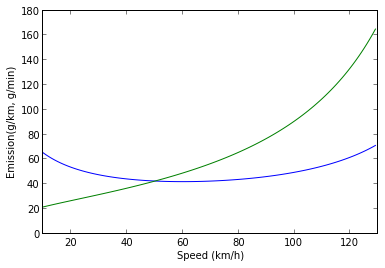
\includegraphics{emission_vs_speed.png}
\caption{{\bf Emission factor as a function of speed. 
g/km blue. g/min green}}
\label{emission_vs_speed}
\end{center}
\end{figure}

The other method uses a measured speed to emission curve and a speed distribution function to estimate the emission. For some pollutants an emission factor function is given, but for pollutants that are directly linked to fuel consumption (i.e. $CO_2$) a fuel consumption function of speed is given (for instance equation \ref{speed}). For $CO_2$ the relationship between emission an fuel consumption is given by the formula \ref{emission_from_fc}.

\begin{equation}\label{emission_from_fc}
E^{CALC}_{co_2}, km = 44,011*\frac{ FC^{CALC}}{12,011 + 1,008 *r_{H:C} + 16,000 * r_{O:C}}
\end{equation}

This formula is based on the assumption that all fuel is consumed, i.e. that each carbon atom in the fuel is oxidised into $CO_2$, which has the molar weight of $44,001$. The numerator $FC^{CALC}$ is the calculated fuel consumption factor, and this is divided with the molar weight of carbon plus the molar weight of hydrogen multiplied with the ratio of hydrogen to carbon ,$r_{H:C}$, plus the molar weight of oxygen multiplied with the ratio of oxygen to carbon, $r_{O:C}$,in the fuel. There are tables for different ratios $r_{H:C}$ and $r_{O:C}$ for different fuel types, given in the COPERT IV methodology guidebook \cite{Ntziachristos2012}.

As an example, passenger vehicles that are regulated by EURO 1 the fuel consumption factor curve is given by equation� \ref{speed}. The coefficients $a$ to $e$ are given for the different engine sizes and pollution regulations. 


\begin{equation}\label{speed}
FC = \frac{a + c*V + e*V^2}{1 + b*V + d*V^2}
\end{equation}
An emission factor (in g/km) versus speed curve can be seen in figure \ref{emission_vs_speed} for a vehicle with engine size less than $1,4 l$  \cite{Mellios2011}, as the blue curve. From the curve it can be seen that the emission factor is larger for low speeds and for high speeds an lowest at moderate speeds (app. 60 km/h). The higher emission factor for low speeds is higher because the engine is underused and therefore not very many kilometres are gained. For higher speeds the opposing forces from wind and friction in bearing, force the engine to work harder, and therefore has a higher emission factor. If instead we look at the emission pr minute, by multiplying the emission curve with the speed, we get the green curve. From the green curve it can be seen that the emission pr time unit is a monotonic growing function, which resembles a second order polynomial. The force of the wind on an object is proportional to the square of the speed.

 The emission is calculated as the integral of the speed distribution multiplied by the emission function as seen in equation \ref{integral}.

\begin{equation}\label{integral}
e_{i,k,r} = \int{e(V)*f_{k,r}(V)dV}
\end{equation}

($i$ is the pollutant for which the emission is calculated, $k$ is the vehicle type, $r$ is the fuel type, $e(V)$ is the emission function of speed, and $f_{k,r}$ is the speed distribution function for the vehicle type $k$ and fuel type $r$).

The data needed to use the Tier 3 method is quite extensive. For each of the 13 vehicle classes (divided by fuel type, vehicle size) activity data for milage for urban, rural and highway travel, hot start/cold start, as well as data for the number of vehicles in each emission regulation is needed. Fortunately the program COPERT IV contains the emission factors, and country specific activity data can be downloaded to use for evaluating national inventories.

This model will form the basis of a complex model for emissions of single trips.

\subsection{Modelling emissions from electric vehicles}
We can calculate the emissions for electric cars by using near real time emission data from Energinet.dk, under the assumption that electric cars will be charged with electricity from the public grid.  There is for now no way to detect if the charging of electric vehicles are not done through the public electric grid, and not for instance by private solar plants.

The dataset from Energinet.dk contains production data for the large power plants, the distributed power plants, wind farms and solar. For each kind of producer, the production is given for east and west Denmark, and the import/export of power to the neighbouring countries is also given. There is data for the temperature and windspeed (for a single location), and an estimated emission factor in $g_{CO_2}/kWh$. The resolution of the data is 5 minutes.
